\documentclass{report}
    \usepackage[utf8]{inputenc}
    \usepackage[ruled,vlined]{algorithm2e}
    \usepackage{amsmath}
    \usepackage{biblatex}
\usepackage{amsthm}
\usepackage[english]{babel}

\newtheorem{theorem}{Theorem}[section]
\newtheorem{corollary}{Corollary}[theorem]
\newtheorem{lemma}[theorem]{Lemma}
% 
\usepackage{tikz}
\usepackage{graphics}
\usepackage{hyperref}
\usetikzlibrary{positioning}
\usetikzlibrary{shapes.geometric}
\addbibresource{References.bib}
    
    \title{
    \line(1,0){350}
    \endgraf\bigskip
    \LARGE\textbf
    {Online graph exploration on trees,unicyclic graphs and cactus graphs}
    \newline
    \line(1,0){350}
    \bigskip
    \bigskip
    }
    
    \author{
    \Large{Md.Mahedi Hasan Rigan}\\
    \Large{Student ID : 1705031}\\\\
    \Large{Asif Mustafa Hassan}\\
    \Large{Student ID : 1705041}
    }
    
    \date{
    \endgraf\bigskip
    \Large{\today}
    }
\begin{document}

\maketitle

\renewcommand{\familydefault}{\sfdefault}
\tableofcontents{}
\chapter{Introduction}
    This report briefly illustrates the well known problem Online graph exploration on different graphs.Online graph exploration is the problem of exploring all vertices of an undirected weighted graph that is initially unknown to the searcher.
    \newline
    \newline
    Normally we work with graphs that we know the edges and vertices.These are known as offline graph.But in online graph we don't know the edges beforehand and we have to traverse all the vertices before starting to the start node. Basically this is similar to Travelling Salesman Problem(TSP).But the only difference between them is in TSP we know the edges value and make efficient choice to traverse the graph.
    \newline
    \newline
    We consider a fixed graph scenario in which a connected undirected graph $G =(V, E)$with $n =|V|$vertices is explored. Each edge $e  \epsilon  E$ has a positive weight |e| and the graph contains a distinguished start node $s  \epsilon     V$from which the searcher begins its explo-ration.We assume that each vertex has an assigned unique identifier (ID).While arriving a vertex for the first time, the searcher obtains the weights of all edges incident to that vertex as well as the IDs of all adjacent vertices.
    \newline \newline
    We will use competitive analysis to measure the performance of an online graph where competitive ratio is the ratio of an online problem solution to its corresponding offline problem solution.So in our case we will get the ratio using travelling salesman problem. We call an online exploration algorithm $c-$competitiveif it produces a tour no longer than $c$ times the optimal (offline) tour for every instance.
    \newline
    \newline
    The best known algorithms on general graphs are Near-est Neighbor (NN) and hierarchical DFS both with a competitive ratio of $\Theta$ $(logn)$. For NN this worst-case ratio is tight even on planar unit-weight (unweighted) graphs. In particular, no algorithm with constant competitive ratio is known on general graphs. On the other hand, the best known lower bound on the competitive ratio of an online algorithm has recently been improved from $2.5$ to $10/3$.We prove that the tight lower bound of $\Theta (logn)$ on the competitive ratio of NN also holds on trees which improves the previous lower bound of $\Theta(logn/ loglogn)$. We do so by modifying a graph construction Hurkens and Woeginger use to prove the lower bound on planar unit-weight graphs.
    \newline
    \chapter{Problem Solving Techniques}
    We are going to mainly focus on two algorithms to solve an online graph exploration on trees, unicyclic grah and cactus graph.These two algorithms are Nearest Neighbour Algorithm and Blocking Algorithm. Here we will discuss Nearest Neighbour Algorithm and Blocking Algorithm as both of them are relevent to our problem.
    \section{Nearest Neighbour Algorithm}
    The nearest neighbour algorithm was one of the first algorithms used to solve the travelling salesman problem approximately. In that problem, the salesman starts at a random city and repeatedly visits the nearest city until all have been visited. The algorithm quickly yields a short tour, but usually not the optimal one.These are the steps of the algorithm:
    \begin{enumerate}
        \item Initialize all vertices as unvisited.
        \item Select an arbitrary vertex, set it as the current vertex u. Mark u as visited.
        \item Find out the shortest edge connecting the current vertex u and an unvisited vertex v.
        \item Set v as the current vertex u. Mark v as visited.
        \item If all the vertices in the domain are visited, then terminate. Else, go to step 3.
    \end{enumerate}
    The sequence of the visited vertices is the output of the algorithm.The nearest neighbour algorithm is easy to implement and executes quickly, but it can sometimes miss shorter routes which are easily noticed with human insight, due to its "greedy" nature. As a general guide, if the last few stages of the tour are comparable in length to the first stages, then the tour is reasonable; if they are much greater, then it is likely that much better tours exist. Another check is to use an algorithm such as the lower bound algorithm to estimate if this tour is good enough.
    \section{Blocking Algorithm}
    The algorithm Blockingδis a generalization of DFS. It uses a blocking condition which, depending on a fixed blocking parameter $\partial$  $\epsilon$  $R$, determines when to delay the traversal of an edge, possibly forever.
    \newline\newline
    \textbf{Definition 2.2.1} (Boundary edge). During the exploration, we call an edge a boundary edge when one of its endpoints has been visited while the other has not.
    \newline\newline
    \textbf{Definition 2.2.2} (Blocking condition).A boundary edge $e =(u, v)$is blocked by another boundary edge $e'=(u', v')$ if eis shorter than $e$ and the length of any shortest path from $u$ to $v'$ is at most $(1 +\partial )|e|$.
    \newline
    \newline
    \begin{algorithm}[H]
    \SetAlgoLined
     \textbf{Input:}A partially explored graph $G$, and a vertex $y$ of $G$ that is explored for the first time.\;
    \While{there is an unblocked boundary edge $e =(u, v)$, with $u$ explored and $v$ unexplored, such that $u =y$ or such that $e$ had previously been blocked by some edge $(u', y)$}{
    walk a shortest known path from $y$ to $u$ \;
    traverse $e =(u, v)$\;
    Blocking $_\partial$ $(G, v)$\;
    walk a shortest known path from $v$ to $y$\;
    
    }
    \caption{The exploration algorithm Blocking $_\partial$ $(G, y)$as in}
    \end{algorithm}
    \bigskip
    On planar graphs, Blocking $_\partial$ is $2(2 +\partial)(1 +2/\partial)$-competitive for $\partial  >0$ and in particular 16-competitive for $\partial=2[4]$. Like in that proof we charge the costs of the algorithms actions to the edges of the explored graph. Let Bδbe the cost of Blockingδ, i.e. the sum of charges to all edges. For each iteration of the while loop, the costs of the movements described in the Lines 2, 3 and 5 are charged to the edge traversed in Line 3. Note that only unblocked boundary edges are charged this way and, in particular, every edge will be charged at most once. Moreover, the following holds.
    
    \chapter{Online graph exploration on trees}
    We recursively define graphs $G_k$ for $k \geq 1$ containing three distinguished vertices $l_k$, $r_k$ and $m_k$. The graph $G_1$ simply consists of the two unit length edges $l_1r_1$and $r_1m_1$. For $k \geq 2$, we construct $G_k$ by placing two copies $G_{k-1}$ and $G_{k-1}$ of $G_{k-1}$next to each other and, in the middle, adding a new vertex $m_k$. To connect the components, we add an edge of length $k$ between $r'_{k-1}$and $l''_{k-1}$as well as a unit weight edge between $l''_{k-1}$and $m_{k}$.
    
    \begin{figure}[h]
        \centering
        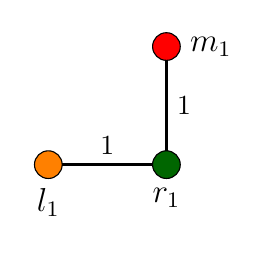
\begin{tikzpicture}[
        node/.style = {
            draw,
            circle,
            fill=gray,
            minimum size = #1,
            inner sep = 0pt,
            outer sep = 0pt
        },  
        node/.default = 6pt,
        node distance = {15mm}
    ]
    {\node[node=10pt, label={[font=\large]below:$l_1$}, fill=orange] (1) {};}
    {\node[node=10pt, label={[font=\large]below:$r_1$}, right of=1, fill=black!60!green] (2) {};}
    {\node[node=10pt, label={[font=\large]right:$m_1$}, above of=2, fill=red] (3) {};}
    \draw[line width = 1pt] (1) -- node[above]{1} (2);
    \draw[line width = 1pt] (2) -- node[right]{1} (3);
    \end{tikzpicture}
    \caption{$G_1$}
    \label{fig:my_label}
    \end{figure}
    
    \begin{figure}[h]
        \centering
        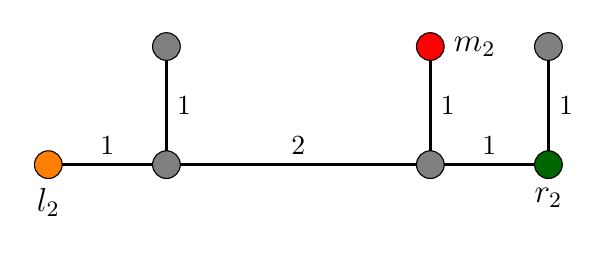
\begin{tikzpicture}[
        node/.style = {
            draw,
            circle,
            fill=gray,
            minimum size = #1,
            inner sep = 0pt,
            outer sep = 0pt
        },  
        node/.default = 6pt,
        node distance = {15mm}
    ]
    \node[node=10pt, label={[font=\large]below:$l_2$}, fill=orange] (1) {};
    \node[node=10pt, right of=1] (2) {};
    \node[node=10pt] (4) [right=30mm of 2] {};
    \node[node=10pt, label={[font=\large]below:$r_2$}, right of=4, fill=black!60!green] (5) {};
    \node[node=10pt, above of=2] (3) {};
    \node[node=10pt, above of=5] (6) {};
    \node[node=10pt, label={[font=\large]right:$m_2$}, fill=red, above of=4] (7) {};
    
    \draw[line width = 1pt] (1) -- node[above]{1} (2);
    \draw[line width = 1pt] (2) -- node[right]{1} (3);
    \draw[line width = 1pt] (4) -- node[above]{1} (5);
    \draw[line width = 1pt] (5) -- node[right]{1} (6);
    
    \draw[line width = 1pt] (2) -- node[above]{2} (4);
    
    \draw[line width = 1pt, node distance = {20mm}] (4) -- node[right]{1} (7); 
    
\end{tikzpicture}
        \caption{$G_2$}
        \label{fig:my_label}
    \end{figure}
    \newpage
    
    \begin{figure}[h]
        \centering
        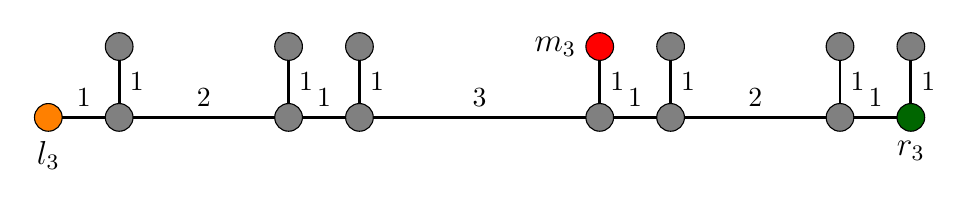
\begin{tikzpicture}[
        node/.style = {
            fill=gray,
            draw,
            circle,
            fill,
            minimum size = #1,
            inner sep = 0pt,
            outer sep = 0pt
        },  
        node/.default = 6pt,
        node distance = {9mm}
    ]
    \node[node=10pt, label={[font=\large]below:$l_3$}, fill=orange] (1) {};
    \node[node=10pt, right of=1] (2) {};
    \node[node=10pt, above of=2] (3) {};
    \node[node=10pt] (4) [right=18mm of 2] {};
    \node[node=10pt, right of=4] (5) {};
    \node[node=10pt, above of=5] (6) {};
    \node[node=10pt, above of=4] (7) {};
    \node[node=10pt] (8) [right=27mm of 5] {};
    \node[node=10pt, right of=8] (9) {};
    \node[node=10pt, above of=9] (10) {};
    \node[node=10pt] (11) [right=18mm of 9] {};
    \node[node=10pt, label={[font=\large]below:$r_3$}, right of=11, fill=black!60!green] (12) {};
    \node[node=10pt, above of=12] (13) {};
    \node[node=10pt, above of=11] (14) {};
    \node[node=10pt, label={[font=\large]left:$m_3$}, above of=8, fill=red] (15) {};
    
    
    
    
    
    
    \draw[line width = 1pt] (1) -- node[above]{1} (2);
    \draw[line width = 1pt] (2) -- node[right]{1} (3);
    \draw[line width = 1pt] (4) -- node[above]{1} (5);
    \draw[line width = 1pt] (5) -- node[right]{1} (6);
    \draw[line width = 1pt] (2) -- node[above]{2} (4);
    \draw[line width = 1pt] (4) -- node[right]{1} (7); 
    \draw[line width = 1pt] (8) -- node[above]{1} (9) ; 
    \draw[line width = 1pt] (9) -- node[right]{1} (10); 
    \draw[line width = 1pt] (9) -- node[above]{2} (11); 
    \draw[line width = 1pt] (11) -- node[above]{1} (12); 
    \draw[line width = 1pt] (12) -- node[right]{1} (13); 
    \draw[line width = 1pt] (11) -- node[right]{1} (14);
    \draw[line width = 1pt] (5) -- node[above]{3}  (8);
    \draw[line width = 1pt] (8) -- node[right]{1} (15);
\end{tikzpicture}
        \caption{$G_3$}
        \label{fig:my_label}
    \end{figure}

    \begin{lemma}
    For {$k\geq1$}, consider a graph {$G$} that contains {$G_k$} as a subgraph. Furthermore, assume that edges between {$G_k$} and {$G-G_k$} are either incident to {$l_k$} and have a length of at least {$1$} or are incident to {$r_k$} and have a length of at least {$k+1$}.
{Then there exists a partial $NN}$ tour exploring all of {$G_k$} that starts in {$l_k$}, finishes in {$m_k$} and has a length of {$$(k+1)*2^k-2$$}}
    \end{lemma}
    \newline
    
    
    
    
    
    
    
    
    
    
    
    
    
    
    
    
    
    
    
    
    
    
    
    
    
    Our goal was to show that the tighter bounds of competitive ratio of NN also holds on the family of the tree.    
\begin{itemize}
    \item {
        The upper bound follows directly from the general case.   
    }
    \item {
        We show that: The lower bound on trees remains same if we follow {$NN$} approach.
    }
\end{itemize}
\newline
%
% 

\begin{figure}[h]
    \centering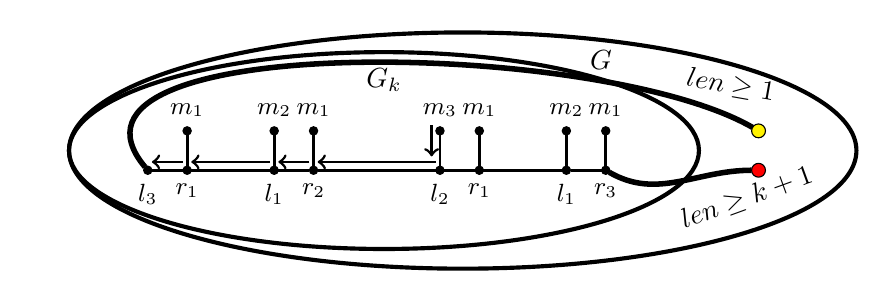
\begin{tikzpicture}[
        node/.style = {
            draw,
            circle,
            fill,
            minimum size = #1,
            inner sep = 0pt,
            outer sep = 0pt
        },  
        node/.default = 6pt,
        node distance = {5mm}
        ]
% 
        \draw[line width=1.5pt] (10,9) arc [start angle=0, end angle=360, x radius=5cm, y radius=1.5cm]
                        node[pos=0.25, yshift=-1em, xshift=5em]{$G$};
        \draw[line width=1.5pt] (8,9) arc [start angle=0, end angle=360, x radius=4cm, y radius=1.25cm]
                        node[pos=0.25, yshift=-1em]{$G_k$};
% 
         \node[node=3pt, label={[font=\small]below:$l_3$}] (1) at (1,8.75) {};
         \node[node=3pt, label={[font=\small]below:$r_1$}, right of=1] (2) {};
         \node[node=3pt, label={[font=\small]above:$m_1$}, above of=2] (3) {};
%  
        \node[node=3pt, label={[font=\small]below:$l_1$}] (4) [right=10mm of 2] {};
% 
% 
        \node[node=3pt, label={[font=\small]below:$r_2$}, right of=4] (5) {};
        \node[node=3pt, label={[font=\small]above:$m_1$}, above of=5] (6) {};
% 
        \node[node=3pt, label={[font=\small]above:$m_2$}, above of=4] (7) {};
% 
% 
        \node[node=3pt, label={[font=\small]below:$l_2$}] (8) [right=15mm of 5] {};
        \node[node=3pt, label={[font=\small]below:$r_1$}, right of=8] (9) {};
        \node[node=3pt, label={[font=\small]above:$m_1$}, above of=9] (10) {};
% 
        \node[node=3pt, label={[font=\small]below:$l_1$}] (11) [right=10mm of 9] {};
% 
        \node[node=3pt, label={[font=\small]below:$r_3$}, right of=11] (12) {};
        \node[node=3pt, label={[font=\small]above:$m_1$}, above of=12] (13) {};
% 
        \node[node=3pt, label={[font=\small]above:$m_2$}, above of=11] (14) {};
% 
        \node[node=3pt, label={[font=\small]above:$m_3$}, above of=8] (15) {};
% 
% 
        \node[node=5pt, fill=red] (G1) [right=18mm of 12]  {};
        \node[node=5pt, fill=yellow] (G2) [right=18mm of 13]  {};
% 
         \draw[line width = 2pt] (1) to [out=130,in=150,looseness=0.75] (G2); 
         \draw[line width = 2pt] (12) to [out=-30,in=180,looseness=1] (G1); 
% 
         \node[above of=G2, xshift=-1em, yshift = 0.2em, rotate = -10] {$len \geq 1$};
         \node[left of=G1, yshift = -1em, xshift = 1em, rotate = 20] {$len \geq k+1$};
% 
% 
% 
        \draw[line width = 1pt  ] (1) -- (2);
        \draw[line width = 1pt  ] (2) -- (3);
% 
        \draw[line width = 1pt  ] (4) -- (5);
        \draw[line width = 1pt  ] (5) -- (6);
% 
        \draw[line width = 1pt  ] (2) -- (4);
        \draw[line width = 1pt  ] (4) -- (7); 
% 
        \draw[line width = 1pt  ] (8) -- (9) ; 
        \draw[line width = 1pt  ] (9) -- (10); 
        \draw[line width = 1pt  ] (9) -- (11); 
        \draw[line width = 1pt  ] (11) --(12); 
        \draw[line width = 1pt  ] (12) --(13); 
        \draw[line width = 1pt  ] (11) --(14);
        \draw[line width = 1pt  ] (5) -- (8);
        \draw[line width = 1pt  ] (8) -- (15);
        
        \draw[->, line width = 1pt  , transform canvas={xshift=-0.3em, yshift=0.35em}] (15) -- (8);
        \draw[->, line width = 1pt  , transform canvas={yshift=0.3em}] (8) -- (5);
        \draw[->, line width = 1pt  , transform canvas={yshift=0.3em}] (5) -- (4);
        \draw[->, line width = 1pt  , transform canvas={yshift=0.3em}] (4) -- (2);
        \draw[->, line width = 1pt  , transform canvas={yshift=0.3em}] (2) -- (1);
        
    \end{tikzpicture}

    \caption{$m_k$ to $l_k$}
    \label{fig:my_label}
\end{figure}





{
Calculating the Competitive Ratio lower bound: 
%
% 
{
% 
%
\begin{itemize}
        \item {
            Traversing graph {$G_k$} when {$G_k$} is a part of larger graph {$G$} with some conditions, the shortest path length from {$l_k$} to {$m_k$} is {$(k+1)*2^k-2$}.
        }
        \item {
            We can use Lemma 1 for only {$G_k$} as we did not need to go outside {$G_k$} in Lemma 1.
        }
        \item {
            Finally complete exploration by returning to {$l_k$} from {$m_k$}.
        }
    \end{itemize}
% 
} 
% 
%
{
% 

% 
    
        {
            {$l_k$} to {$m_k$} needs length: \qquad {$(k+1)*2^k-2$}      
        }
        {
            {$m_k$} to {$l_k$} needs length: 
            \begin{align*}
                Ret(G_k)    &= 1 + k + p_{k-1} \\
                            &= 1 + k + (2^k - (k-1) - 2) \\
                            &= 1 + k + 2^k - k + 1 - 2 = 2^k 
            \end{align*}
        }
    
% 
} 
% 
% 

}

\begin{theorem}
The competitive ratio of NN on trees is $\Theta(logn)$.
\end{theorem}
\textbf{Proof}: Total length for complete exploration on Online Tree {$G_k$}:
\begin{align*}
                NN(G_k) &= Ret(G_k) + (k+1)*2^k - 2 \\
                        &= 2^k + (k+1)*2^k - 2 \\
                        &= (k+2)*2^k - 2 \\
\end{align*}

{
        The {NN} approach on particular Online Tree family has length: 
            $$(k+2)*2^k-2$$
}
{
        The optimal solution on this offline Tree family should have length: 
            \begin{align*}
                OPT(G_k) &= 2*w_k \\
                         &= 6*2^k - 2k - 6
            \end{align*}
    }
{
          {$G_k$} has vertices:
          \begin{align*}
              n_k &= 2^{k+1}-1 \\ 
              2^{k+1} &= n_k + 1 \\ 
              log_2{2^{k+1}} &= log_2{(n_k + 1)} \\ 
              k + 1 &= log_2{(n_k + 1)} \\ 
              k &= log_2{(n_k + 1)} - 1 
          \end{align*}
}

So, Lower bound: 
        \begin{align*}
            c   &= \frac{NN(G_k)}{OPT(G_k)} \\
                &= \frac{(k+2)*2^k - 2}{6*2^k - 2k - 6} \\
                &\geq \frac{k+2}{6} \\
                &= \frac{\log_2{(n+1)}+1}{6} \qed  
        \end{align*}



\chapter{Conclusion}
Online explorations are common in practical life. Moreover, online tree explorations help robots determine their path in unknown situations and much more. It is extremely important yet does not seem useful from a theoretical point of view. 
Although, this problem looks quite similar to TSP(Travelling Salesman Problem), it can be solved in polynomial time upon defining the environment family. A large number of tree family can be defined for polynomial online exploration domain. We can think of a future where most of the graphs will be online explorable in polynomial time, enhancing our robots and much more.

\nocite{*}                                          
\printbibliography
\end{document}
